
\begin{center}
\Huge
Cirkler og cirklens ligning
\end{center}
\section*{Cirklens ligning}
\stepcounter{section}

Hvis vi har en linje $l$, så kan vi finde en ligning, der beskriver alle de punkter, der ligger på linjen. Det samme kan vi gøre for cirkler. Ligningen for en cirkel kaldes naturligt nok for \textit{cirklens ligning}, og for at bestemme ligningen for en cirkel skal vi kende dens midtpunkt og dens radius. Dette er beskrevet i følgende sætning.
\begin{setn}[Cirklens ligning]
Ethvert punkt $(x,y)$ ligger på cirklen $c$ med radius $r$ og centrum i $(x_0,y_0)$ præcist når det er opfyldt, at 
\begin{align*}
(x-x_0)^2+(y-y_0)^2 = r^2.
\end{align*}
\end{setn}
\begin{proof}
Punktet $(x,y)$ ligger på cirklen præcist i de tilfælde, hvor vektoren 
\begin{align*}
\begin{pmatrix}
x-x_0 \\ y-y_0
\end{pmatrix}
\end{align*}
har længde $r$. Dette er ensbetydende med, at 
\begin{align*}
\left|\begin{pmatrix}
x-x_0 \\ y-y_0
\end{pmatrix}\right| = r \ &\Leftrightarrow \ \sqrt{(x-x_0)^2+(y-y_0)^2} = r \\
&\Leftrightarrow \ (x-x_0)^2+(y-y_0)^2 = r^2.
\end{align*}
\end{proof}

\begin{exa}
Vi betragter cirklen på Fig. \ref{fig:cirkel}. Den har centrum i punktet $(1,1)$ og radius $2$. Derfor lyder cirklens ligning for denne cirkel
\begin{align*}
(x-1)^2 + (y-1)^2 = 4.
\end{align*}
\begin{figure}[H]
\centering
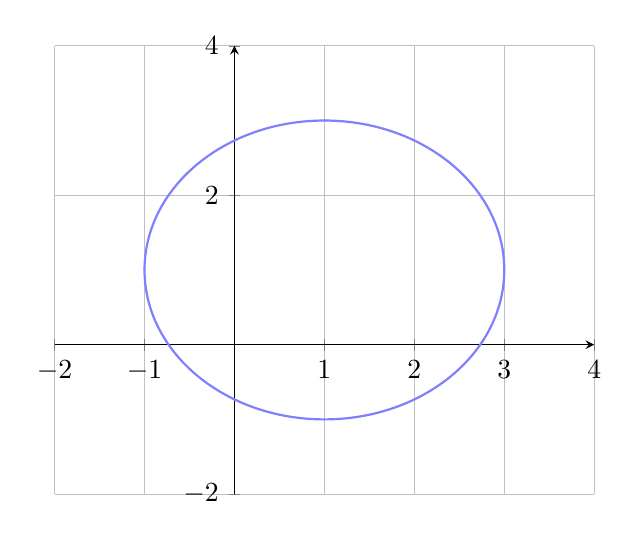
\begin{tikzpicture}
\begin{axis}[axis lines = middle, xmin = -2, xmax = 4, ymin = -2, ymax = 4,
grid = both
]
\draw[color = blue!50, thick]  (axis cs:1,1) circle (2);
\end{axis}
\end{tikzpicture}
\caption{Cirkel}
\label{fig:cirkel}
\end{figure}
\end{exa}

\begin{exa}
Vi betragter cirklen på Fig. \ref{fig:cirkel2}. Vi skal bestemme de tangenter til cirklen, der har hældning -1. Dette gøres i Geogebra (\href{https://github.com/ChristianJLex/TeachingNotes/raw/master/Diverse/Geogebra/Cirkeltangenter.ggb}{\color{blue!60} Link til fil}), og tangenterne findes til at have ligningerne 
\begin{align*}
y = -x+5 
\end{align*}
og
\begin{align*}
y = -x +1, 
\end{align*}
som vi kan se på figuren.
\begin{figure}[H]
\centering
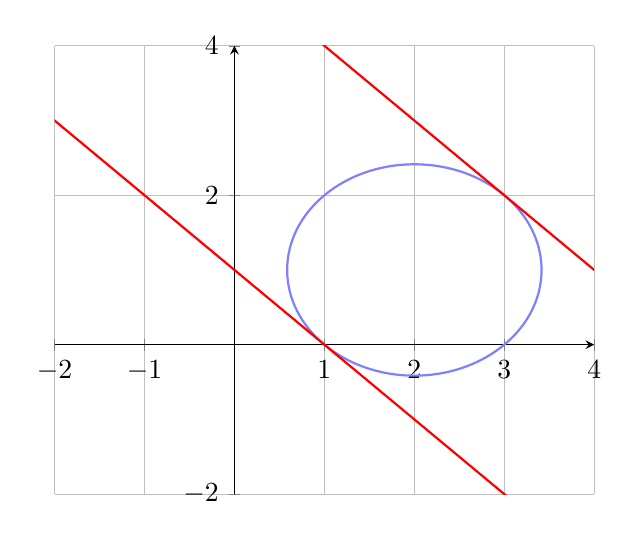
\begin{tikzpicture}
\begin{axis}[axis lines = middle, xmin = -2, xmax = 4, ymin = -2, ymax = 4,
grid = both
]
\draw[color = blue!50, thick]  (axis cs:2,1) circle (1.41421356237);
\addplot[color = red, thick] {-x+5};
\addplot[color = red, thick] {-x+1};
\end{axis}
\end{tikzpicture}
\caption{Cirkel}
\label{fig:cirkel2}
\end{figure}
\end{exa}

\section*{Opgave 1}
Bestem ligningerne for følgende cirkler
\begin{figure}[H]
\centering
\resizebox{0.45\textwidth}{0.45\textwidth}
{
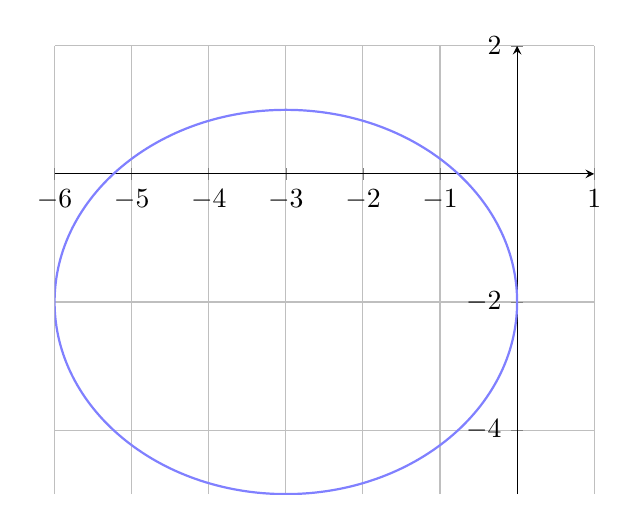
\begin{tikzpicture}
\begin{axis}[axis lines = middle, xmin = -6, xmax = 1, ymin = -5, ymax = 2,
grid = both]
\draw[color = blue!50, thick]  (axis cs:-3,-2) circle (3);
\end{axis}
\end{tikzpicture}
}
\resizebox{0.45\textwidth}{0.45\textwidth}
{
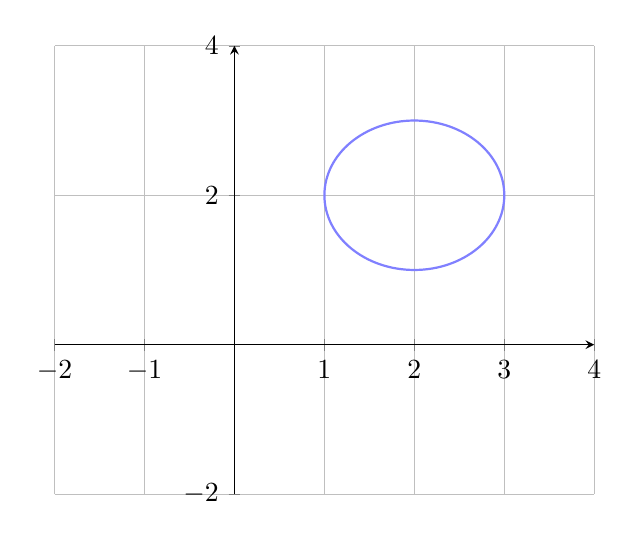
\begin{tikzpicture}
\begin{axis}[axis lines = middle, xmin = -2, xmax = 4, ymin = -2, ymax = 4,
grid = both]
\draw[color = blue!50, thick]  (axis cs:2,2) circle (1);
\end{axis}
\end{tikzpicture}
}
\resizebox{0.45\textwidth}{0.45\textwidth}
{
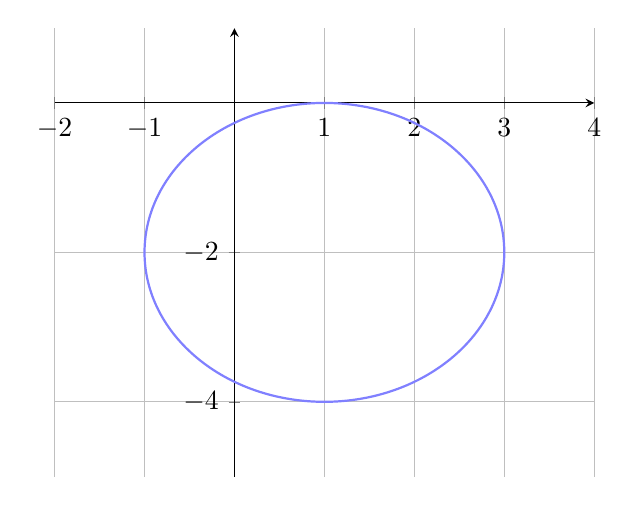
\begin{tikzpicture}
\begin{axis}[axis lines = middle, xmin = -2, xmax = 4, ymin = -5, ymax = 1,
grid = both]
\draw[color = blue!50, thick]  (axis cs:1,-2) circle (2);
\end{axis}
\end{tikzpicture}
}
\resizebox{0.45\textwidth}{0.45\textwidth}
{
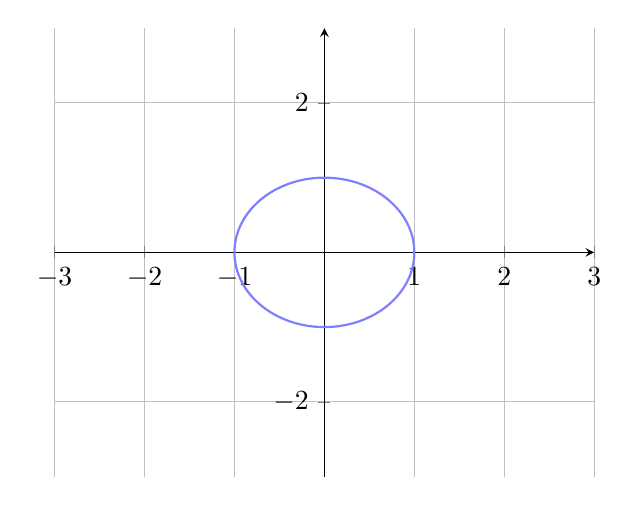
\begin{tikzpicture}
\begin{axis}[axis lines = middle, xmin = -3, xmax = 3, ymin = -3, ymax = 3,
grid = both]
\draw[color = blue!50, thick]  (axis cs:0,0) circle (1);
\end{axis}
\end{tikzpicture}
}
\resizebox{0.45\textwidth}{0.45\textwidth}
{
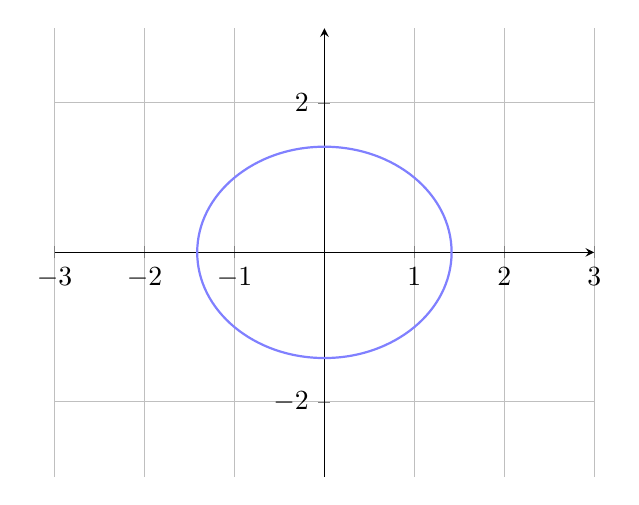
\begin{tikzpicture}
\begin{axis}[axis lines = middle, xmin = -3, xmax = 3, ymin = -3, ymax = 3,
grid = both]
\draw[color = blue!50, thick]  (axis cs:0,0) circle (1.4142135623);
\end{axis}
\end{tikzpicture}
}
\resizebox{0.45\textwidth}{0.45\textwidth}
{
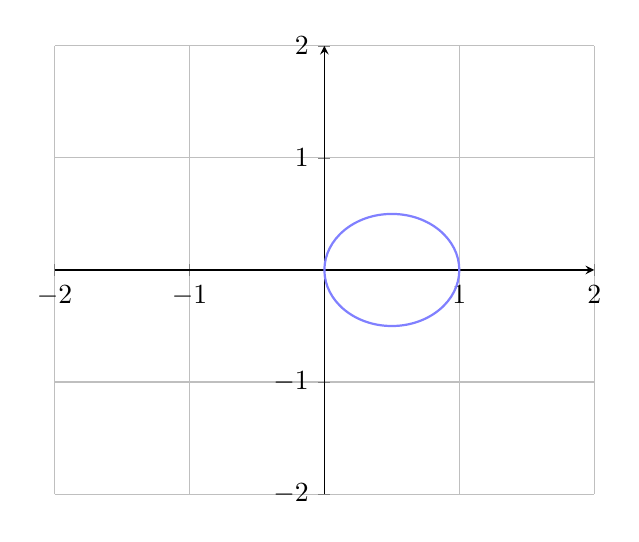
\begin{tikzpicture}
\begin{axis}[axis lines = middle, xmin = -2, xmax = 2, ymin = -2, ymax = 2,
grid = both]
\draw[color = blue!50, thick]  (axis cs:0.5,0) circle (0.5);
\end{axis}
\end{tikzpicture}
}
\caption{Cirkler}
\label{fig:cirkler}
\end{figure}

\section*{Opgave 2}
\begin{enumerate}[label=\roman*)]
\item En cirkel har ligningen $(x-2)^2+(y+3)^2 = 4$, og en linje har ligningen 
\begin{align*}
y=2x-1.
\end{align*}
Bestem skæringen mellem linjen og cirklen i Geogebra. 
\item En cirkel har ligningen $x^2+y^2-1=0$. Bestem de tangenter, der har hældning $0$ til cirklen i Geogebra. 
\item En cirkel har ligningen $(x+1)^2 +(y-1)^2 = 9$, og et punkt $(-4,1)$ ligger på cirklen. Bestem ligningen for tangenten til cirklen i dette punkt i Geogebra. 
\end{enumerate}
\section*{Opgave 3}
Aflevering